\documentclass[1p]{elsarticle_modified}
%\bibliographystyle{elsarticle-num}

%\usepackage[colorlinks]{hyperref}
%\usepackage{abbrmath_seonhwa} %\Abb, \Ascr, \Acal ,\Abf, \Afrak
\usepackage{amsfonts}
\usepackage{amssymb}
\usepackage{amsmath}
\usepackage{amsthm}
\usepackage{scalefnt}
\usepackage{amsbsy}
\usepackage{kotex}
\usepackage{caption}
\usepackage{subfig}
\usepackage{color}
\usepackage{graphicx}
\usepackage{xcolor} %% white, black, red, green, blue, cyan, magenta, yellow
\usepackage{float}
\usepackage{setspace}
\usepackage{hyperref}

\usepackage{tikz}
\usetikzlibrary{arrows}

\usepackage{multirow}
\usepackage{array} % fixed length table
\usepackage{hhline}

%%%%%%%%%%%%%%%%%%%%%
\makeatletter
\renewcommand*\env@matrix[1][\arraystretch]{%
	\edef\arraystretch{#1}%
	\hskip -\arraycolsep
	\let\@ifnextchar\new@ifnextchar
	\array{*\c@MaxMatrixCols c}}
\makeatother %https://tex.stackexchange.com/questions/14071/how-can-i-increase-the-line-spacing-in-a-matrix
%%%%%%%%%%%%%%%

\usepackage[normalem]{ulem}

\newcommand{\msout}[1]{\ifmmode\text{\sout{\ensuremath{#1}}}\else\sout{#1}\fi}
%SOURCE: \msout is \stkout macro in https://tex.stackexchange.com/questions/20609/strikeout-in-math-mode

\newcommand{\cancel}[1]{
	\ifmmode
	{\color{red}\msout{#1}}
	\else
	{\color{red}\sout{#1}}
	\fi
}

\newcommand{\add}[1]{
	{\color{blue}\uwave{#1}}
}

\newcommand{\replace}[2]{
	\ifmmode
	{\color{red}\msout{#1}}{\color{blue}\uwave{#2}}
	\else
	{\color{red}\sout{#1}}{\color{blue}\uwave{#2}}
	\fi
}

\newcommand{\Sol}{\mathcal{S}} %segment
\newcommand{\D}{D} %diagram
\newcommand{\A}{\mathcal{A}} %arc


%%%%%%%%%%%%%%%%%%%%%%%%%%%%%5 test

\def\sl{\operatorname{\textup{SL}}(2,\Cbb)}
\def\psl{\operatorname{\textup{PSL}}(2,\Cbb)}
\def\quan{\mkern 1mu \triangleright \mkern 1mu}

\theoremstyle{definition}
\newtheorem{thm}{Theorem}[section]
\newtheorem{prop}[thm]{Proposition}
\newtheorem{lem}[thm]{Lemma}
\newtheorem{ques}[thm]{Question}
\newtheorem{cor}[thm]{Corollary}
\newtheorem{defn}[thm]{Definition}
\newtheorem{exam}[thm]{Example}
\newtheorem{rmk}[thm]{Remark}
\newtheorem{alg}[thm]{Algorithm}

\newcommand{\I}{\sqrt{-1}}
\begin{document}

%\begin{frontmatter}
%
%\title{Boundary parabolic representations of knots up to 8 crossings}
%
%%% Group authors per affiliation:
%\author{Yunhi Cho} 
%\address{Department of Mathematics, University of Seoul, Seoul, Korea}
%\ead{yhcho@uos.ac.kr}
%
%
%\author{Seonhwa Kim} %\fnref{s_kim}}
%\address{Center for Geometry and Physics, Institute for Basic Science, Pohang, 37673, Korea}
%\ead{ryeona17@ibs.re.kr}
%
%\author{Hyuk Kim}
%\address{Department of Mathematical Sciences, Seoul National University, Seoul 08826, Korea}
%\ead{hyukkim@snu.ac.kr}
%
%\author{Seokbeom Yoon}
%\address{Department of Mathematical Sciences, Seoul National University, Seoul, 08826,  Korea}
%\ead{sbyoon15@snu.ac.kr}
%
%\begin{abstract}
%We find all boundary parabolic representation of knots up to 8 crossings.
%
%\end{abstract}
%\begin{keyword}
%    \MSC[2010] 57M25 
%\end{keyword}
%
%\end{frontmatter}

%\linenumbers
%\tableofcontents
%
\newcommand\colored[1]{\textcolor{white}{\rule[-0.35ex]{0.8em}{1.4ex}}\kern-0.8em\color{red} #1}%
%\newcommand\colored[1]{\textcolor{white}{ #1}\kern-2.17ex	\textcolor{white}{ #1}\kern-1.81ex	\textcolor{white}{ #1}\kern-2.15ex\color{red}#1	}

{\Large $\underline{11n_{167}~(K11n_{167})}$}

\setlength{\tabcolsep}{10pt}
\renewcommand{\arraystretch}{1.6}
\vspace{1cm}\begin{tabular}{m{100pt}>{\centering\arraybackslash}m{274pt}}
\multirow{5}{120pt}{
	\centering
	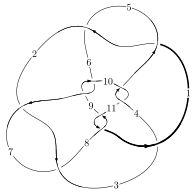
\includegraphics[width=112pt]{../../../GIT/diagram.site/Diagrams/png/783_11n_167.png}\\
\ \ \ A knot diagram\footnotemark}&
\allowdisplaybreaks
\textbf{Linearized knot diagam} \\
\cline{2-2}
 &
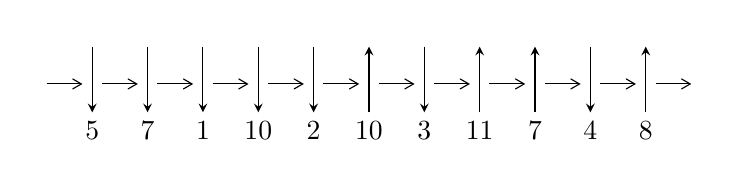
\begin{tikzpicture}[x=20pt, y=17pt]
	% nodes
	\node (C0) at (0, 0) {};
	\node (C1) at (1, 0) {};
	\node (C1U) at (1, +1) {};
	\node (C1D) at (1, -1) {5};

	\node (C2) at (2, 0) {};
	\node (C2U) at (2, +1) {};
	\node (C2D) at (2, -1) {7};

	\node (C3) at (3, 0) {};
	\node (C3U) at (3, +1) {};
	\node (C3D) at (3, -1) {1};

	\node (C4) at (4, 0) {};
	\node (C4U) at (4, +1) {};
	\node (C4D) at (4, -1) {10};

	\node (C5) at (5, 0) {};
	\node (C5U) at (5, +1) {};
	\node (C5D) at (5, -1) {2};

	\node (C6) at (6, 0) {};
	\node (C6U) at (6, +1) {};
	\node (C6D) at (6, -1) {10};

	\node (C7) at (7, 0) {};
	\node (C7U) at (7, +1) {};
	\node (C7D) at (7, -1) {3};

	\node (C8) at (8, 0) {};
	\node (C8U) at (8, +1) {};
	\node (C8D) at (8, -1) {11};

	\node (C9) at (9, 0) {};
	\node (C9U) at (9, +1) {};
	\node (C9D) at (9, -1) {7};

	\node (C10) at (10, 0) {};
	\node (C10U) at (10, +1) {};
	\node (C10D) at (10, -1) {4};

	\node (C11) at (11, 0) {};
	\node (C11U) at (11, +1) {};
	\node (C11D) at (11, -1) {8};
	\node (C12) at (12, 0) {};

	% arrows
	\draw[->,>={angle 60}]
	(C0) edge (C1) (C1) edge (C2) (C2) edge (C3) (C3) edge (C4) (C4) edge (C5) (C5) edge (C6) (C6) edge (C7) (C7) edge (C8) (C8) edge (C9) (C9) edge (C10) (C10) edge (C11) (C11) edge (C12) ;	\draw[->,>=stealth]
	(C1U) edge (C1D) (C2U) edge (C2D) (C3U) edge (C3D) (C4U) edge (C4D) (C5U) edge (C5D) (C6D) edge (C6U) (C7U) edge (C7D) (C8D) edge (C8U) (C9D) edge (C9U) (C10U) edge (C10D) (C11D) edge (C11U) ;
	\end{tikzpicture} \\
\hhline{~~} \\& 
\textbf{Solving Sequence} \\ \cline{2-2} 
 &
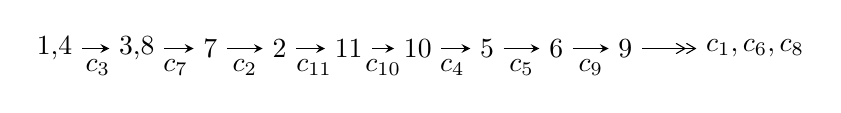
\begin{tikzpicture}[x=25pt, y=7pt]
	% node
	\node (A0) at (-1/8, 0) {1,4};
	\node (A1) at (17/16, 0) {3,8};
	\node (A2) at (17/8, 0) {7};
	\node (A3) at (25/8, 0) {2};
	\node (A4) at (33/8, 0) {11};
	\node (A5) at (41/8, 0) {10};
	\node (A6) at (49/8, 0) {5};
	\node (A7) at (57/8, 0) {6};
	\node (A8) at (65/8, 0) {9};
	\node (C1) at (1/2, -1) {$c_{3}$};
	\node (C2) at (13/8, -1) {$c_{7}$};
	\node (C3) at (21/8, -1) {$c_{2}$};
	\node (C4) at (29/8, -1) {$c_{11}$};
	\node (C5) at (37/8, -1) {$c_{10}$};
	\node (C6) at (45/8, -1) {$c_{4}$};
	\node (C7) at (53/8, -1) {$c_{5}$};
	\node (C8) at (61/8, -1) {$c_{9}$};
	\node (A9) at (10, 0) {$c_{1},c_{6},c_{8}$};

	% edge
	\draw[->,>=stealth]	
	(A0) edge (A1) (A1) edge (A2) (A2) edge (A3) (A3) edge (A4) (A4) edge (A5) (A5) edge (A6) (A6) edge (A7) (A7) edge (A8) ;
	\draw[->>,>={angle 60}]	
	(A8) edge (A9);
\end{tikzpicture} \\ 

\end{tabular} \\

\footnotetext{
The image of knot diagram is generated by the software ``\textbf{Draw programme}" developed by Andrew Bartholomew(\url{http://www.layer8.co.uk/maths/draw/index.htm\#Running-draw}), where we modified some parts for our purpose(\url{https://github.com/CATsTAILs/LinksPainter}).
}\phantom \\ \newline 
\centering \textbf{Ideals for irreducible components\footnotemark of $X_{\text{par}}$} 
 
\begin{align*}
I^u_{1}&=\langle 
-22089881 u^{18}-37947869 u^{17}+\cdots+242489462 b+98525885,\\
\phantom{I^u_{1}}&\phantom{= \langle  }-61574971 u^{18}+98525885 u^{17}+\cdots+242489462 a+1067204433,\;u^{19}-8 u^{17}+\cdots-5 u+1\rangle \\
I^u_{2}&=\langle 
1.77398\times10^{18} u^{23}+2.26651\times10^{18} u^{22}+\cdots+4.24873\times10^{18} b-7.44747\times10^{18},\\
\phantom{I^u_{2}}&\phantom{= \langle  }-1.90928\times10^{19} u^{23}-2.27388\times10^{19} u^{22}+\cdots+2.12437\times10^{19} a+1.14920\times10^{20},\;u^{24}+u^{23}+\cdots-8 u+2\rangle \\
I^u_{3}&=\langle 
- u^7+u^6+2 u^5- u^3- u^2+b-2 u-1,\;- u^6+u^5+u^4+a-2,\;u^8-2 u^6-2 u^5+u^3+3 u^2+3 u+1\rangle \\
I^u_{4}&=\langle 
- u^3- u^2+b-1,\;u^3+2 u^2+2 a+u,\;u^4+2 u^3- u^2-2 u+2\rangle \\
\\
\end{align*}
\raggedright * 4 irreducible components of $\dim_{\mathbb{C}}=0$, with total 55 representations.\\
\footnotetext{All coefficients of polynomials are rational numbers. But the coefficients are sometimes approximated in decimal forms when there is not enough margin.}
\newpage
\renewcommand{\arraystretch}{1}
\centering \section*{I. $I^u_{1}= \langle -2.21\times10^{7} u^{18}-3.79\times10^{7} u^{17}+\cdots+2.42\times10^{8} b+9.85\times10^{7},\;-6.16\times10^{7} u^{18}+9.85\times10^{7} u^{17}+\cdots+2.42\times10^{8} a+1.07\times10^{9},\;u^{19}-8 u^{17}+\cdots-5 u+1 \rangle$}
\flushleft \textbf{(i) Arc colorings}\\
\begin{tabular}{m{7pt} m{180pt} m{7pt} m{180pt} }
\flushright $a_{1}=$&$\begin{pmatrix}0\\u\end{pmatrix}$ \\
\flushright $a_{4}=$&$\begin{pmatrix}1\\0\end{pmatrix}$ \\
\flushright $a_{3}=$&$\begin{pmatrix}1\\- u^2\end{pmatrix}$ \\
\flushright $a_{8}=$&$\begin{pmatrix}0.253928 u^{18}-0.406310 u^{17}+\cdots-1.98160 u-4.40103\\0.0910963 u^{18}+0.156493 u^{17}+\cdots+3.28548 u-0.406310\end{pmatrix}$ \\
\flushright $a_{7}=$&$\begin{pmatrix}0.253928 u^{18}-0.406310 u^{17}+\cdots-0.981600 u-4.40103\\0.0910963 u^{18}+0.156493 u^{17}+\cdots+3.28548 u-0.406310\end{pmatrix}$ \\
\flushright $a_{2}=$&$\begin{pmatrix}0.406310 u^{18}+0.0910963 u^{17}+\cdots+3.13139 u+1.25393\\-0.156493 u^{18}-0.188283 u^{17}+\cdots-0.0491713 u+0.0910963\end{pmatrix}$ \\
\flushright $a_{11}=$&$\begin{pmatrix}-0.610280 u^{18}-0.343192 u^{17}+\cdots-10.3730 u-2.60824\\0.370173 u^{18}+0.142628 u^{17}+\cdots+4.39116 u-0.749502\end{pmatrix}$ \\
\flushright $a_{10}=$&$\begin{pmatrix}-0.240107 u^{18}-0.200564 u^{17}+\cdots-5.98180 u-3.35775\\0.370173 u^{18}+0.142628 u^{17}+\cdots+4.39116 u-0.749502\end{pmatrix}$ \\
\flushright $a_{5}=$&$\begin{pmatrix}-0.655534 u^{18}-0.0971700 u^{17}+\cdots-12.7360 u+2.59475\\-0.0593229 u^{18}-0.229893 u^{17}+\cdots+0.633751 u-0.564438\end{pmatrix}$ \\
\flushright $a_{6}=$&$\begin{pmatrix}-1.21860 u^{18}+0.176434 u^{17}+\cdots-14.2029 u+4.08632\\0.00607376 u^{18}-0.198103 u^{17}+\cdots-1.60256 u-0.249224\end{pmatrix}$ \\
\flushright $a_{9}=$&$\begin{pmatrix}-0.365855 u^{18}-0.499533 u^{17}+\cdots-17.4546 u-5.30364\\0.418084 u^{18}-0.0169879 u^{17}+\cdots+6.52297 u-1.24903\end{pmatrix}$\\ \flushright $a_{9}=$&$\begin{pmatrix}-0.365855 u^{18}-0.499533 u^{17}+\cdots-17.4546 u-5.30364\\0.418084 u^{18}-0.0169879 u^{17}+\cdots+6.52297 u-1.24903\end{pmatrix}$\\&\end{tabular}
\flushleft \textbf{(ii) Obstruction class $= -1$}\\~\\
\flushleft \textbf{(iii) Cusp Shapes $= -\frac{261922646}{121244731} u^{18}+\frac{40889015}{121244731} u^{17}+\cdots+\frac{452208248}{121244731} u+\frac{720534416}{121244731}$}\\~\\
\newpage\renewcommand{\arraystretch}{1}
\flushleft \textbf{(iv) u-Polynomials at the component}\newline \\
\begin{tabular}{m{50pt}|m{274pt}}
Crossings & \hspace{64pt}u-Polynomials at each crossing \\
\hline $$\begin{aligned}c_{1},c_{5}\end{aligned}$$&$\begin{aligned}
&u^{19}+8 u^{18}+\cdots+13 u+2
\end{aligned}$\\
\hline $$\begin{aligned}c_{2},c_{3},c_{7}\end{aligned}$$&$\begin{aligned}
&u^{19}-8 u^{17}+\cdots-5 u+1
\end{aligned}$\\
\hline $$\begin{aligned}c_{4},c_{10}\end{aligned}$$&$\begin{aligned}
&u^{19}+8 u^{17}+\cdots+4 u+1
\end{aligned}$\\
\hline $$\begin{aligned}c_{6},c_{9}\end{aligned}$$&$\begin{aligned}
&u^{19}+2 u^{18}+\cdots+11 u+2
\end{aligned}$\\
\hline $$\begin{aligned}c_{8},c_{11}\end{aligned}$$&$\begin{aligned}
&u^{19}+7 u^{18}+\cdots+47 u+4
\end{aligned}$\\
\hline
\end{tabular}\\~\\
\newpage\renewcommand{\arraystretch}{1}
\flushleft \textbf{(v) Riley Polynomials at the component}\newline \\
\begin{tabular}{m{50pt}|m{274pt}}
Crossings & \hspace{64pt}Riley Polynomials at each crossing \\
\hline $$\begin{aligned}c_{1},c_{5}\end{aligned}$$&$\begin{aligned}
&y^{19}-4 y^{18}+\cdots-27 y-4
\end{aligned}$\\
\hline $$\begin{aligned}c_{2},c_{3},c_{7}\end{aligned}$$&$\begin{aligned}
&y^{19}-16 y^{18}+\cdots+19 y-1
\end{aligned}$\\
\hline $$\begin{aligned}c_{4},c_{10}\end{aligned}$$&$\begin{aligned}
&y^{19}+16 y^{18}+\cdots-12 y-1
\end{aligned}$\\
\hline $$\begin{aligned}c_{6},c_{9}\end{aligned}$$&$\begin{aligned}
&y^{19}-16 y^{18}+\cdots+81 y-4
\end{aligned}$\\
\hline $$\begin{aligned}c_{8},c_{11}\end{aligned}$$&$\begin{aligned}
&y^{19}+7 y^{18}+\cdots+1025 y-16
\end{aligned}$\\
\hline
\end{tabular}\\~\\
\newpage\flushleft \textbf{(vi) Complex Volumes and Cusp Shapes}
$$\begin{array}{c|c|c}  
\text{Solutions to }I^u_{1}& \I (\text{vol} + \sqrt{-1}CS) & \text{Cusp shape}\\
 \hline 
\begin{aligned}
u &= -0.953283 + 0.590186 I \\
a &= \phantom{-}0.497813 - 0.825854 I \\
b &= -0.30300 + 1.61317 I\end{aligned}
 & -3.36214 + 0.48881 I & -6.63793 - 2.65665 I \\ \hline\begin{aligned}
u &= -0.953283 - 0.590186 I \\
a &= \phantom{-}0.497813 + 0.825854 I \\
b &= -0.30300 - 1.61317 I\end{aligned}
 & -3.36214 - 0.48881 I & -6.63793 + 2.65665 I \\ \hline\begin{aligned}
u &= \phantom{-}0.978082 + 0.672701 I \\
a &= \phantom{-}1.070170 - 0.278653 I \\
b &= \phantom{-}0.071909 - 0.595075 I\end{aligned}
 & \phantom{-}5.37613 - 7.26815 I & -2.70960 + 5.48443 I \\ \hline\begin{aligned}
u &= \phantom{-}0.978082 - 0.672701 I \\
a &= \phantom{-}1.070170 + 0.278653 I \\
b &= \phantom{-}0.071909 + 0.595075 I\end{aligned}
 & \phantom{-}5.37613 + 7.26815 I & -2.70960 - 5.48443 I \\ \hline\begin{aligned}
u &= -1.124820 + 0.396400 I \\
a &= \phantom{-}0.225058 - 0.730978 I \\
b &= -0.72235 + 1.40708 I\end{aligned}
 & -3.09782 + 0.05780 I & -6.02643 + 0.15389 I \\ \hline\begin{aligned}
u &= -1.124820 - 0.396400 I \\
a &= \phantom{-}0.225058 + 0.730978 I \\
b &= -0.72235 - 1.40708 I\end{aligned}
 & -3.09782 - 0.05780 I & -6.02643 - 0.15389 I \\ \hline\begin{aligned}
u &= -1.054220 + 0.617800 I \\
a &= -1.066300 + 0.064508 I \\
b &= -0.360174 - 0.818216 I\end{aligned}
 & \phantom{-}4.51703 - 0.89042 I & -2.37683 + 0.17113 I \\ \hline\begin{aligned}
u &= -1.054220 - 0.617800 I \\
a &= -1.066300 - 0.064508 I \\
b &= -0.360174 + 0.818216 I\end{aligned}
 & \phantom{-}4.51703 + 0.89042 I & -2.37683 - 0.17113 I \\ \hline\begin{aligned}
u &= \phantom{-}0.741245 + 0.208527 I \\
a &= -0.51834 - 1.73606 I \\
b &= \phantom{-}0.466823 + 1.247140 I\end{aligned}
 & -2.65661 + 3.10000 I & -6.27419 - 4.22218 I \\ \hline\begin{aligned}
u &= \phantom{-}0.741245 - 0.208527 I \\
a &= -0.51834 + 1.73606 I \\
b &= \phantom{-}0.466823 - 1.247140 I\end{aligned}
 & -2.65661 - 3.10000 I & -6.27419 + 4.22218 I\\
 \hline 
 \end{array}$$\newpage$$\begin{array}{c|c|c}  
\text{Solutions to }I^u_{1}& \I (\text{vol} + \sqrt{-1}CS) & \text{Cusp shape}\\
 \hline 
\begin{aligned}
u &= \phantom{-}1.46886 + 0.25961 I \\
a &= \phantom{-}0.273323 - 0.690530 I \\
b &= \phantom{-}0.37094 + 1.49448 I\end{aligned}
 & -8.71916 - 2.37470 I & -12.53850 - 4.28279 I \\ \hline\begin{aligned}
u &= \phantom{-}1.46886 - 0.25961 I \\
a &= \phantom{-}0.273323 + 0.690530 I \\
b &= \phantom{-}0.37094 - 1.49448 I\end{aligned}
 & -8.71916 + 2.37470 I & -12.53850 + 4.28279 I \\ \hline\begin{aligned}
u &= -0.477001\phantom{ +0.000000I} \\
a &= -0.253883\phantom{ +0.000000I} \\
b &= -0.419235\phantom{ +0.000000I}\end{aligned}
 & -0.803589\phantom{ +0.000000I} & -12.4280\phantom{ +0.000000I} \\ \hline\begin{aligned}
u &= -1.39506 + 0.83246 I \\
a &= -0.053021 - 0.851335 I \\
b &= \phantom{-}0.64874 + 1.77620 I\end{aligned}
 & \phantom{-}3.02325 + 5.91409 I & -2.64836 - 3.66933 I \\ \hline\begin{aligned}
u &= -1.39506 - 0.83246 I \\
a &= -0.053021 + 0.851335 I \\
b &= \phantom{-}0.64874 - 1.77620 I\end{aligned}
 & \phantom{-}3.02325 - 5.91409 I & -2.64836 + 3.66933 I \\ \hline\begin{aligned}
u &= \phantom{-}1.38951 + 0.89919 I \\
a &= -0.052745 - 0.891369 I \\
b &= -0.77871 + 2.03128 I\end{aligned}
 & \phantom{-}2.6009 - 14.2087 I & -4.30199 + 7.64083 I \\ \hline\begin{aligned}
u &= \phantom{-}1.38951 - 0.89919 I \\
a &= -0.052745 + 0.891369 I \\
b &= -0.77871 - 2.03128 I\end{aligned}
 & \phantom{-}2.6009 + 14.2087 I & -4.30199 - 7.64083 I \\ \hline\begin{aligned}
u &= \phantom{-}0.188175 + 0.151731 I \\
a &= -4.24902 + 1.30686 I \\
b &= \phantom{-}0.315435 + 0.378179 I\end{aligned}
 & \phantom{-}1.89777 + 1.11232 I & \phantom{-}4.22795 - 4.88598 I \\ \hline\begin{aligned}
u &= \phantom{-}0.188175 - 0.151731 I \\
a &= -4.24902 - 1.30686 I \\
b &= \phantom{-}0.315435 - 0.378179 I\end{aligned}
 & \phantom{-}1.89777 - 1.11232 I & \phantom{-}4.22795 + 4.88598 I\\
 \hline 
 \end{array}$$\newpage\newpage\renewcommand{\arraystretch}{1}
\centering \section*{II. $I^u_{2}= \langle 1.77\times10^{18} u^{23}+2.27\times10^{18} u^{22}+\cdots+4.25\times10^{18} b-7.45\times10^{18},\;-1.91\times10^{19} u^{23}-2.27\times10^{19} u^{22}+\cdots+2.12\times10^{19} a+1.15\times10^{20},\;u^{24}+u^{23}+\cdots-8 u+2 \rangle$}
\flushleft \textbf{(i) Arc colorings}\\
\begin{tabular}{m{7pt} m{180pt} m{7pt} m{180pt} }
\flushright $a_{1}=$&$\begin{pmatrix}0\\u\end{pmatrix}$ \\
\flushright $a_{4}=$&$\begin{pmatrix}1\\0\end{pmatrix}$ \\
\flushright $a_{3}=$&$\begin{pmatrix}1\\- u^2\end{pmatrix}$ \\
\flushright $a_{8}=$&$\begin{pmatrix}0.898752 u^{23}+1.07038 u^{22}+\cdots+12.0912 u-5.40961\\-0.417531 u^{23}-0.533456 u^{22}+\cdots-3.66675 u+1.75287\end{pmatrix}$ \\
\flushright $a_{7}=$&$\begin{pmatrix}\frac{1}{2} u^{23}+\frac{1}{2} u^{22}+\cdots+8 u-4\\-0.398752 u^{23}-0.570379 u^{22}+\cdots-3.09123 u+1.40961\end{pmatrix}$ \\
\flushright $a_{2}=$&$\begin{pmatrix}-0.704807 u^{23}-1.10356 u^{22}+\cdots-6.67794 u+2.54722\\-0.244696 u^{23}-0.273474 u^{22}+\cdots-2.26972 u+0.601506\end{pmatrix}$ \\
\flushright $a_{11}=$&$\begin{pmatrix}1.24995 u^{23}+1.72388 u^{22}+\cdots+14.2509 u-5.98658\\-0.507773 u^{23}-0.801281 u^{22}+\cdots-2.45122 u+1.52483\end{pmatrix}$ \\
\flushright $a_{10}=$&$\begin{pmatrix}0.742173 u^{23}+0.922597 u^{22}+\cdots+11.7997 u-4.46175\\-0.507773 u^{23}-0.801281 u^{22}+\cdots-2.45122 u+1.52483\end{pmatrix}$ \\
\flushright $a_{5}=$&$\begin{pmatrix}0.239284 u^{23}+0.478472 u^{22}+\cdots+2.29165 u-1.06026\\-0.596088 u^{23}-0.741810 u^{22}+\cdots-5.97824 u+2.40135\end{pmatrix}$ \\
\flushright $a_{6}=$&$\begin{pmatrix}0.359990 u^{23}+0.826922 u^{22}+\cdots+1.48988 u-0.206011\\-0.282468 u^{23}-0.307556 u^{22}+\cdots-2.91950 u+1.66220\end{pmatrix}$ \\
\flushright $a_{9}=$&$\begin{pmatrix}2.18922 u^{23}+3.04082 u^{22}+\cdots+25.5796 u-11.0724\\-0.844038 u^{23}-1.26644 u^{22}+\cdots-5.33860 u+3.13224\end{pmatrix}$\\ \flushright $a_{9}=$&$\begin{pmatrix}2.18922 u^{23}+3.04082 u^{22}+\cdots+25.5796 u-11.0724\\-0.844038 u^{23}-1.26644 u^{22}+\cdots-5.33860 u+3.13224\end{pmatrix}$\\&\end{tabular}
\flushleft \textbf{(ii) Obstruction class $= -1$}\\~\\
\flushleft \textbf{(iii) Cusp Shapes $= \frac{4484056006391387816}{2124366145116320153} u^{23}+\frac{6874045510728739710}{2124366145116320153} u^{22}+\cdots+\frac{19962270314208126262}{2124366145116320153} u-\frac{11397374893510619150}{2124366145116320153}$}\\~\\
\newpage\renewcommand{\arraystretch}{1}
\flushleft \textbf{(iv) u-Polynomials at the component}\newline \\
\begin{tabular}{m{50pt}|m{274pt}}
Crossings & \hspace{64pt}u-Polynomials at each crossing \\
\hline $$\begin{aligned}c_{1},c_{5}\end{aligned}$$&$\begin{aligned}
&(u^{12}-3 u^{11}+\cdots-3 u+1)^{2}
\end{aligned}$\\
\hline $$\begin{aligned}c_{2},c_{3},c_{7}\end{aligned}$$&$\begin{aligned}
&u^{24}+u^{23}+\cdots-8 u+2
\end{aligned}$\\
\hline $$\begin{aligned}c_{4},c_{10}\end{aligned}$$&$\begin{aligned}
&u^{24}+u^{23}+\cdots-60 u+10
\end{aligned}$\\
\hline $$\begin{aligned}c_{6},c_{9}\end{aligned}$$&$\begin{aligned}
&u^{24}+3 u^{23}+\cdots+192 u+17
\end{aligned}$\\
\hline $$\begin{aligned}c_{8},c_{11}\end{aligned}$$&$\begin{aligned}
&(u^{12}-3 u^{11}+\cdots-5 u+3)^{2}
\end{aligned}$\\
\hline
\end{tabular}\\~\\
\newpage\renewcommand{\arraystretch}{1}
\flushleft \textbf{(v) Riley Polynomials at the component}\newline \\
\begin{tabular}{m{50pt}|m{274pt}}
Crossings & \hspace{64pt}Riley Polynomials at each crossing \\
\hline $$\begin{aligned}c_{1},c_{5}\end{aligned}$$&$\begin{aligned}
&(y^{12}- y^{11}+\cdots+3 y+1)^{2}
\end{aligned}$\\
\hline $$\begin{aligned}c_{2},c_{3},c_{7}\end{aligned}$$&$\begin{aligned}
&y^{24}-3 y^{23}+\cdots-36 y^2+4
\end{aligned}$\\
\hline $$\begin{aligned}c_{4},c_{10}\end{aligned}$$&$\begin{aligned}
&y^{24}+21 y^{23}+\cdots+3560 y+100
\end{aligned}$\\
\hline $$\begin{aligned}c_{6},c_{9}\end{aligned}$$&$\begin{aligned}
&y^{24}-21 y^{23}+\cdots-16090 y+289
\end{aligned}$\\
\hline $$\begin{aligned}c_{8},c_{11}\end{aligned}$$&$\begin{aligned}
&(y^{12}+7 y^{11}+\cdots+35 y+9)^{2}
\end{aligned}$\\
\hline
\end{tabular}\\~\\
\newpage\flushleft \textbf{(vi) Complex Volumes and Cusp Shapes}
$$\begin{array}{c|c|c}  
\text{Solutions to }I^u_{2}& \I (\text{vol} + \sqrt{-1}CS) & \text{Cusp shape}\\
 \hline 
\begin{aligned}
u &= -0.787408 + 0.597220 I \\
a &= \phantom{-}0.219391 - 0.993794 I \\
b &= \phantom{-}1.46372 + 2.07332 I\end{aligned}
 & \phantom{-}5.39798 + 5.66008 I & -4.22997 - 6.14268 I \\ \hline\begin{aligned}
u &= -0.787408 - 0.597220 I \\
a &= \phantom{-}0.219391 + 0.993794 I \\
b &= \phantom{-}1.46372 - 2.07332 I\end{aligned}
 & \phantom{-}5.39798 - 5.66008 I & -4.22997 + 6.14268 I \\ \hline\begin{aligned}
u &= -0.600013 + 0.769421 I \\
a &= -0.539028 + 1.257780 I \\
b &= -0.117110 - 0.655487 I\end{aligned}
 & -0.77344 + 4.75233 I & -0.57550 - 5.65227 I \\ \hline\begin{aligned}
u &= -0.600013 - 0.769421 I \\
a &= -0.539028 - 1.257780 I \\
b &= -0.117110 + 0.655487 I\end{aligned}
 & -0.77344 - 4.75233 I & -0.57550 + 5.65227 I \\ \hline\begin{aligned}
u &= \phantom{-}0.920865 + 0.478649 I \\
a &= \phantom{-}0.235557 + 1.372650 I \\
b &= -0.02624 - 1.98543 I\end{aligned}
 & -3.09418 - 6.13442 I & -10.3699 + 10.2596 I \\ \hline\begin{aligned}
u &= \phantom{-}0.920865 - 0.478649 I \\
a &= \phantom{-}0.235557 - 1.372650 I \\
b &= -0.02624 + 1.98543 I\end{aligned}
 & -3.09418 + 6.13442 I & -10.3699 - 10.2596 I \\ \hline\begin{aligned}
u &= \phantom{-}0.839992 + 0.703903 I \\
a &= -0.124749 - 0.804667 I \\
b &= -1.49997 + 1.70732 I\end{aligned}
 & \phantom{-}5.86114 + 1.98712 I & -2.94340 + 1.27592 I \\ \hline\begin{aligned}
u &= \phantom{-}0.839992 - 0.703903 I \\
a &= -0.124749 + 0.804667 I \\
b &= -1.49997 - 1.70732 I\end{aligned}
 & \phantom{-}5.86114 - 1.98712 I & -2.94340 - 1.27592 I \\ \hline\begin{aligned}
u &= \phantom{-}1.169280 + 0.449583 I \\
a &= -0.145064 + 1.055900 I \\
b &= \phantom{-}0.67915 - 1.84712 I\end{aligned}
 & -0.77344 - 4.75233 I & -0.57550 + 5.65227 I \\ \hline\begin{aligned}
u &= \phantom{-}1.169280 - 0.449583 I \\
a &= -0.145064 - 1.055900 I \\
b &= \phantom{-}0.67915 + 1.84712 I\end{aligned}
 & -0.77344 + 4.75233 I & -0.57550 - 5.65227 I\\
 \hline 
 \end{array}$$\newpage$$\begin{array}{c|c|c}  
\text{Solutions to }I^u_{2}& \I (\text{vol} + \sqrt{-1}CS) & \text{Cusp shape}\\
 \hline 
\begin{aligned}
u &= \phantom{-}0.418416 + 0.516472 I \\
a &= \phantom{-}0.80019 + 1.21965 I \\
b &= -1.146740 - 0.284708 I\end{aligned}
 & -4.41600 - 1.23001 I & -6.02056 + 5.25591 I \\ \hline\begin{aligned}
u &= \phantom{-}0.418416 - 0.516472 I \\
a &= \phantom{-}0.80019 - 1.21965 I \\
b &= -1.146740 + 0.284708 I\end{aligned}
 & -4.41600 + 1.23001 I & -6.02056 - 5.25591 I \\ \hline\begin{aligned}
u &= -1.09051 + 0.92826 I \\
a &= -0.389136 + 0.931266 I \\
b &= -0.83707 - 1.57150 I\end{aligned}
 & -3.09418 + 6.13442 I & -10.3699 - 10.2596 I \\ \hline\begin{aligned}
u &= -1.09051 - 0.92826 I \\
a &= -0.389136 - 0.931266 I \\
b &= -0.83707 + 1.57150 I\end{aligned}
 & -3.09418 - 6.13442 I & -10.3699 + 10.2596 I \\ \hline\begin{aligned}
u &= \phantom{-}0.488121 + 0.138133 I \\
a &= -1.77306 + 0.99449 I \\
b &= \phantom{-}0.399018 - 0.436599 I\end{aligned}
 & \phantom{-}1.95930 - 1.10762 I & \phantom{-}2.13937 + 5.92060 I \\ \hline\begin{aligned}
u &= \phantom{-}0.488121 - 0.138133 I \\
a &= -1.77306 - 0.99449 I \\
b &= \phantom{-}0.399018 + 0.436599 I\end{aligned}
 & \phantom{-}1.95930 + 1.10762 I & \phantom{-}2.13937 - 5.92060 I \\ \hline\begin{aligned}
u &= -0.57462 + 1.39073 I \\
a &= -0.586220 - 0.089711 I \\
b &= \phantom{-}0.043111 - 0.376940 I\end{aligned}
 & \phantom{-}5.86114 + 1.98712 I & -2.94340 + 1.27592 I \\ \hline\begin{aligned}
u &= -0.57462 - 1.39073 I \\
a &= -0.586220 + 0.089711 I \\
b &= \phantom{-}0.043111 + 0.376940 I\end{aligned}
 & \phantom{-}5.86114 - 1.98712 I & -2.94340 - 1.27592 I \\ \hline\begin{aligned}
u &= -0.123712 + 0.457725 I \\
a &= \phantom{-}0.06216 + 2.17412 I \\
b &= \phantom{-}0.253968 + 0.291137 I\end{aligned}
 & \phantom{-}1.95930 + 1.10762 I & \phantom{-}2.13937 - 5.92060 I \\ \hline\begin{aligned}
u &= -0.123712 - 0.457725 I \\
a &= \phantom{-}0.06216 - 2.17412 I \\
b &= \phantom{-}0.253968 - 0.291137 I\end{aligned}
 & \phantom{-}1.95930 - 1.10762 I & \phantom{-}2.13937 + 5.92060 I\\
 \hline 
 \end{array}$$\newpage$$\begin{array}{c|c|c}  
\text{Solutions to }I^u_{2}& \I (\text{vol} + \sqrt{-1}CS) & \text{Cusp shape}\\
 \hline 
\begin{aligned}
u &= \phantom{-}0.58682 + 1.60527 I \\
a &= \phantom{-}0.586529 - 0.047705 I \\
b &= \phantom{-}0.432171 - 0.614303 I\end{aligned}
 & \phantom{-}5.39798 + 5.66008 I & -4.22997 - 6.14268 I \\ \hline\begin{aligned}
u &= \phantom{-}0.58682 - 1.60527 I \\
a &= \phantom{-}0.586529 + 0.047705 I \\
b &= \phantom{-}0.432171 + 0.614303 I\end{aligned}
 & \phantom{-}5.39798 - 5.66008 I & -4.22997 + 6.14268 I \\ \hline\begin{aligned}
u &= -1.74722 + 0.05067 I \\
a &= \phantom{-}0.153439 + 0.533057 I \\
b &= -0.14400 - 2.11524 I\end{aligned}
 & -4.41600 + 1.23001 I & -6.02056 - 5.25591 I \\ \hline\begin{aligned}
u &= -1.74722 - 0.05067 I \\
a &= \phantom{-}0.153439 - 0.533057 I \\
b &= -0.14400 + 2.11524 I\end{aligned}
 & -4.41600 - 1.23001 I & -6.02056 + 5.25591 I\\
 \hline 
 \end{array}$$\newpage\newpage\renewcommand{\arraystretch}{1}
\centering \section*{III. $I^u_{3}= \langle - u^7+u^6+2 u^5- u^3- u^2+b-2 u-1,\;- u^6+u^5+u^4+a-2,\;u^8-2 u^6-2 u^5+u^3+3 u^2+3 u+1 \rangle$}
\flushleft \textbf{(i) Arc colorings}\\
\begin{tabular}{m{7pt} m{180pt} m{7pt} m{180pt} }
\flushright $a_{1}=$&$\begin{pmatrix}0\\u\end{pmatrix}$ \\
\flushright $a_{4}=$&$\begin{pmatrix}1\\0\end{pmatrix}$ \\
\flushright $a_{3}=$&$\begin{pmatrix}1\\- u^2\end{pmatrix}$ \\
\flushright $a_{8}=$&$\begin{pmatrix}u^6- u^5- u^4+2\\u^7- u^6-2 u^5+u^3+u^2+2 u+1\end{pmatrix}$ \\
\flushright $a_{7}=$&$\begin{pmatrix}u^6- u^5- u^4- u+2\\u^7- u^6-2 u^5+2 u^3+u^2+2 u+1\end{pmatrix}$ \\
\flushright $a_{2}=$&$\begin{pmatrix}u^7- u^6- u^5- u^2+2 u+1\\- u^7+2 u^5+2 u^4-2 u^2-2 u-1\end{pmatrix}$ \\
\flushright $a_{11}=$&$\begin{pmatrix}- u^7+2 u^6- u^3-2 u+1\\u^7- u^6- u^5- u^4+u^2+3 u+1\end{pmatrix}$ \\
\flushright $a_{10}=$&$\begin{pmatrix}u^6- u^5- u^4- u^3+u^2+u+2\\u^7- u^6- u^5- u^4+u^2+3 u+1\end{pmatrix}$ \\
\flushright $a_{5}=$&$\begin{pmatrix}2 u^7- u^6-4 u^5-2 u^4+2 u^3+2 u^2+5 u+3\\u^2- u-1\end{pmatrix}$ \\
\flushright $a_{6}=$&$\begin{pmatrix}2 u^7- u^6-4 u^5- u^4+2 u^3+3 u+3\\- u^6+2 u^4+2 u^3-2 u-1\end{pmatrix}$ \\
\flushright $a_{9}=$&$\begin{pmatrix}-2 u^7+3 u^6+u^5+u^4-2 u^3-5 u+1\\2 u^7-2 u^6-3 u^5- u^4+2 u^3+u^2+4 u+2\end{pmatrix}$\\ \flushright $a_{9}=$&$\begin{pmatrix}-2 u^7+3 u^6+u^5+u^4-2 u^3-5 u+1\\2 u^7-2 u^6-3 u^5- u^4+2 u^3+u^2+4 u+2\end{pmatrix}$\\&\end{tabular}
\flushleft \textbf{(ii) Obstruction class $= 1$}\\~\\
\flushleft \textbf{(iii) Cusp Shapes $= -5 u^7+u^6+12 u^5+9 u^4-4 u^3-6 u^2-18 u-18$}\\~\\
\newpage\renewcommand{\arraystretch}{1}
\flushleft \textbf{(iv) u-Polynomials at the component}\newline \\
\begin{tabular}{m{50pt}|m{274pt}}
Crossings & \hspace{64pt}u-Polynomials at each crossing \\
\hline $$\begin{aligned}c_{1}\end{aligned}$$&$\begin{aligned}
&u^8+5 u^7+10 u^6+10 u^5+5 u^4+3 u^3+4 u^2+2 u+1
\end{aligned}$\\
\hline $$\begin{aligned}c_{2}\end{aligned}$$&$\begin{aligned}
&u^8-2 u^6+2 u^5- u^3+3 u^2-3 u+1
\end{aligned}$\\
\hline $$\begin{aligned}c_{3},c_{7}\end{aligned}$$&$\begin{aligned}
&u^8-2 u^6-2 u^5+u^3+3 u^2+3 u+1
\end{aligned}$\\
\hline $$\begin{aligned}c_{4}\end{aligned}$$&$\begin{aligned}
&u^8+2 u^6- u^5+2 u^4+2 u^3+4 u^2+2 u+1
\end{aligned}$\\
\hline $$\begin{aligned}c_{5}\end{aligned}$$&$\begin{aligned}
&u^8-5 u^7+10 u^6-10 u^5+5 u^4-3 u^3+4 u^2-2 u+1
\end{aligned}$\\
\hline $$\begin{aligned}c_{6}\end{aligned}$$&$\begin{aligned}
&u^8+2 u^7-2 u^6-6 u^5+5 u^3+u^2- u+1
\end{aligned}$\\
\hline $$\begin{aligned}c_{8}\end{aligned}$$&$\begin{aligned}
&u^8+4 u^7+9 u^6+12 u^5+9 u^4+2 u^3-2 u^2- u+1
\end{aligned}$\\
\hline $$\begin{aligned}c_{9}\end{aligned}$$&$\begin{aligned}
&u^8-2 u^7-2 u^6+6 u^5-5 u^3+u^2+u+1
\end{aligned}$\\
\hline $$\begin{aligned}c_{10}\end{aligned}$$&$\begin{aligned}
&u^8+2 u^6+u^5+2 u^4-2 u^3+4 u^2-2 u+1
\end{aligned}$\\
\hline $$\begin{aligned}c_{11}\end{aligned}$$&$\begin{aligned}
&u^8-4 u^7+9 u^6-12 u^5+9 u^4-2 u^3-2 u^2+u+1
\end{aligned}$\\
\hline
\end{tabular}\\~\\
\newpage\renewcommand{\arraystretch}{1}
\flushleft \textbf{(v) Riley Polynomials at the component}\newline \\
\begin{tabular}{m{50pt}|m{274pt}}
Crossings & \hspace{64pt}Riley Polynomials at each crossing \\
\hline $$\begin{aligned}c_{1},c_{5}\end{aligned}$$&$\begin{aligned}
&y^8-5 y^7+10 y^6-22 y^5+27 y^4+11 y^3+14 y^2+4 y+1
\end{aligned}$\\
\hline $$\begin{aligned}c_{2},c_{3},c_{7}\end{aligned}$$&$\begin{aligned}
&y^8-4 y^7+4 y^6+2 y^5-6 y^4+7 y^3+3 y^2-3 y+1
\end{aligned}$\\
\hline $$\begin{aligned}c_{4},c_{10}\end{aligned}$$&$\begin{aligned}
&y^8+4 y^7+8 y^6+15 y^5+26 y^4+20 y^3+12 y^2+4 y+1
\end{aligned}$\\
\hline $$\begin{aligned}c_{6},c_{9}\end{aligned}$$&$\begin{aligned}
&y^8-8 y^7+28 y^6-54 y^5+62 y^4-41 y^3+11 y^2+y+1
\end{aligned}$\\
\hline $$\begin{aligned}c_{8},c_{11}\end{aligned}$$&$\begin{aligned}
&y^8+2 y^7+3 y^6-2 y^5+7 y^4+2 y^3+26 y^2-5 y+1
\end{aligned}$\\
\hline
\end{tabular}\\~\\
\newpage\flushleft \textbf{(vi) Complex Volumes and Cusp Shapes}
$$\begin{array}{c|c|c}  
\text{Solutions to }I^u_{3}& \I (\text{vol} + \sqrt{-1}CS) & \text{Cusp shape}\\
 \hline 
\begin{aligned}
u &= \phantom{-}0.047355 + 0.955386 I \\
a &= \phantom{-}0.250346 - 0.387349 I \\
b &= \phantom{-}0.145540 - 1.330730 I\end{aligned}
 & \phantom{-}5.86099 + 3.83824 I & -2.61527 - 2.77290 I \\ \hline\begin{aligned}
u &= \phantom{-}0.047355 - 0.955386 I \\
a &= \phantom{-}0.250346 + 0.387349 I \\
b &= \phantom{-}0.145540 + 1.330730 I\end{aligned}
 & \phantom{-}5.86099 - 3.83824 I & -2.61527 + 2.77290 I \\ \hline\begin{aligned}
u &= -0.923072 + 0.606984 I \\
a &= -0.288078 + 1.324400 I \\
b &= -0.42170 - 1.57032 I\end{aligned}
 & -2.20821 + 5.58533 I & -2.91572 - 6.03344 I \\ \hline\begin{aligned}
u &= -0.923072 - 0.606984 I \\
a &= -0.288078 - 1.324400 I \\
b &= -0.42170 + 1.57032 I\end{aligned}
 & -2.20821 - 5.58533 I & -2.91572 + 6.03344 I \\ \hline\begin{aligned}
u &= -0.595163 + 0.229046 I \\
a &= \phantom{-}1.91573 + 0.00857 I \\
b &= \phantom{-}0.014742 + 0.290671 I\end{aligned}
 & \phantom{-}1.46644 - 0.78325 I & -8.36606 - 3.84221 I \\ \hline\begin{aligned}
u &= -0.595163 - 0.229046 I \\
a &= \phantom{-}1.91573 - 0.00857 I \\
b &= \phantom{-}0.014742 - 0.290671 I\end{aligned}
 & \phantom{-}1.46644 + 0.78325 I & -8.36606 + 3.84221 I \\ \hline\begin{aligned}
u &= \phantom{-}1.47088 + 0.19586 I \\
a &= -0.377996 + 0.744591 I \\
b &= -0.23859 - 1.56042 I\end{aligned}
 & -8.40909 - 2.81417 I & -3.60294 + 7.34570 I \\ \hline\begin{aligned}
u &= \phantom{-}1.47088 - 0.19586 I \\
a &= -0.377996 - 0.744591 I \\
b &= -0.23859 + 1.56042 I\end{aligned}
 & -8.40909 + 2.81417 I & -3.60294 - 7.34570 I\\
 \hline 
 \end{array}$$\newpage\newpage\renewcommand{\arraystretch}{1}
\centering \section*{IV. $I^u_{4}= \langle - u^3- u^2+b-1,\;u^3+2 u^2+2 a+u,\;u^4+2 u^3- u^2-2 u+2 \rangle$}
\flushleft \textbf{(i) Arc colorings}\\
\begin{tabular}{m{7pt} m{180pt} m{7pt} m{180pt} }
\flushright $a_{1}=$&$\begin{pmatrix}0\\u\end{pmatrix}$ \\
\flushright $a_{4}=$&$\begin{pmatrix}1\\0\end{pmatrix}$ \\
\flushright $a_{3}=$&$\begin{pmatrix}1\\- u^2\end{pmatrix}$ \\
\flushright $a_{8}=$&$\begin{pmatrix}-\frac{1}{2} u^3- u^2-\frac{1}{2} u\\u^3+u^2+1\end{pmatrix}$ \\
\flushright $a_{7}=$&$\begin{pmatrix}-\frac{1}{2} u^3- u^2+\frac{1}{2} u+1\\1\end{pmatrix}$ \\
\flushright $a_{2}=$&$\begin{pmatrix}\frac{1}{2} u^3+u^2-\frac{1}{2} u-1\\- u^2- u-1\end{pmatrix}$ \\
\flushright $a_{11}=$&$\begin{pmatrix}-\frac{1}{2} u^3- u^2+\frac{1}{2} u+1\\u^3+2 u^2-1\end{pmatrix}$ \\
\flushright $a_{10}=$&$\begin{pmatrix}\frac{1}{2} u^3+u^2+\frac{1}{2} u\\u^3+2 u^2-1\end{pmatrix}$ \\
\flushright $a_{5}=$&$\begin{pmatrix}\frac{1}{2} u^3+u^2-\frac{1}{2} u-1\\- u^2-2 u-1\end{pmatrix}$ \\
\flushright $a_{6}=$&$\begin{pmatrix}0\\- u\end{pmatrix}$ \\
\flushright $a_{9}=$&$\begin{pmatrix}0\\u^3+u^2- u\end{pmatrix}$\\ \flushright $a_{9}=$&$\begin{pmatrix}0\\u^3+u^2- u\end{pmatrix}$\\&\end{tabular}
\flushleft \textbf{(ii) Obstruction class $= 1$}\\~\\
\flushleft \textbf{(iii) Cusp Shapes $= -12$}\\~\\
\newpage\renewcommand{\arraystretch}{1}
\flushleft \textbf{(iv) u-Polynomials at the component}\newline \\
\begin{tabular}{m{50pt}|m{274pt}}
Crossings & \hspace{64pt}u-Polynomials at each crossing \\
\hline $$\begin{aligned}c_{1}\end{aligned}$$&$\begin{aligned}
&(u-1)^4
\end{aligned}$\\
\hline $$\begin{aligned}c_{2}\end{aligned}$$&$\begin{aligned}
&u^4-2 u^3- u^2+2 u+2
\end{aligned}$\\
\hline $$\begin{aligned}c_{3},c_{7}\end{aligned}$$&$\begin{aligned}
&u^4+2 u^3- u^2-2 u+2
\end{aligned}$\\
\hline $$\begin{aligned}c_{4}\end{aligned}$$&$\begin{aligned}
&u^4+3 u^2-2 u+2
\end{aligned}$\\
\hline $$\begin{aligned}c_{5}\end{aligned}$$&$\begin{aligned}
&(u+1)^4
\end{aligned}$\\
\hline $$\begin{aligned}c_{6},c_{8},c_{9}\\c_{11}\end{aligned}$$&$\begin{aligned}
&(u^2+1)^2
\end{aligned}$\\
\hline $$\begin{aligned}c_{10}\end{aligned}$$&$\begin{aligned}
&u^4+3 u^2+2 u+2
\end{aligned}$\\
\hline
\end{tabular}\\~\\
\newpage\renewcommand{\arraystretch}{1}
\flushleft \textbf{(v) Riley Polynomials at the component}\newline \\
\begin{tabular}{m{50pt}|m{274pt}}
Crossings & \hspace{64pt}Riley Polynomials at each crossing \\
\hline $$\begin{aligned}c_{1},c_{5}\end{aligned}$$&$\begin{aligned}
&(y-1)^4
\end{aligned}$\\
\hline $$\begin{aligned}c_{2},c_{3},c_{7}\end{aligned}$$&$\begin{aligned}
&y^4-6 y^3+13 y^2-8 y+4
\end{aligned}$\\
\hline $$\begin{aligned}c_{4},c_{10}\end{aligned}$$&$\begin{aligned}
&y^4+6 y^3+13 y^2+8 y+4
\end{aligned}$\\
\hline $$\begin{aligned}c_{6},c_{8},c_{9}\\c_{11}\end{aligned}$$&$\begin{aligned}
&(y+1)^4
\end{aligned}$\\
\hline
\end{tabular}\\~\\
\newpage\flushleft \textbf{(vi) Complex Volumes and Cusp Shapes}
$$\begin{array}{c|c|c}  
\text{Solutions to }I^u_{4}& \I (\text{vol} + \sqrt{-1}CS) & \text{Cusp shape}\\
 \hline 
\begin{aligned}
u &= \phantom{-}0.693897 + 0.418797 I \\
a &= -0.637550 - 1.056350 I \\
b &= \phantom{-}1.27510 + 1.11269 I\end{aligned}
 & -4.93480\phantom{ +0.000000I} & -12.0000\phantom{ +0.000000I} \\ \hline\begin{aligned}
u &= \phantom{-}0.693897 - 0.418797 I \\
a &= -0.637550 + 1.056350 I \\
b &= \phantom{-}1.27510 - 1.11269 I\end{aligned}
 & -4.93480\phantom{ +0.000000I} & -12.0000\phantom{ +0.000000I} \\ \hline\begin{aligned}
u &= -1.69390 + 0.41880 I \\
a &= \phantom{-}0.137550 - 0.556347 I \\
b &= -0.27510 + 2.11269 I\end{aligned}
 & -4.93480\phantom{ +0.000000I} & -12.0000\phantom{ +0.000000I} \\ \hline\begin{aligned}
u &= -1.69390 - 0.41880 I \\
a &= \phantom{-}0.137550 + 0.556347 I \\
b &= -0.27510 - 2.11269 I\end{aligned}
 & -4.93480\phantom{ +0.000000I} & -12.0000\phantom{ +0.000000I}\\
 \hline 
 \end{array}$$\newpage
\newpage\renewcommand{\arraystretch}{1}
\centering \section*{ V. u-Polynomials}
\begin{tabular}{m{50pt}|m{274pt}}
Crossings & \hspace{64pt}u-Polynomials at each crossing \\
\hline $$\begin{aligned}c_{1}\end{aligned}$$&$\begin{aligned}
&(u-1)^4(u^8+5 u^7+10 u^6+10 u^5+5 u^4+3 u^3+4 u^2+2 u+1)\\
&\cdot((u^{12}-3 u^{11}+\cdots-3 u+1)^{2})(u^{19}+8 u^{18}+\cdots+13 u+2)
\end{aligned}$\\
\hline $$\begin{aligned}c_{2}\end{aligned}$$&$\begin{aligned}
&(u^4-2 u^3- u^2+2 u+2)(u^8-2 u^6+2 u^5- u^3+3 u^2-3 u+1)\\
&\cdot(u^{19}-8 u^{17}+\cdots-5 u+1)(u^{24}+u^{23}+\cdots-8 u+2)
\end{aligned}$\\
\hline $$\begin{aligned}c_{3},c_{7}\end{aligned}$$&$\begin{aligned}
&(u^4+2 u^3- u^2-2 u+2)(u^8-2 u^6-2 u^5+u^3+3 u^2+3 u+1)\\
&\cdot(u^{19}-8 u^{17}+\cdots-5 u+1)(u^{24}+u^{23}+\cdots-8 u+2)
\end{aligned}$\\
\hline $$\begin{aligned}c_{4}\end{aligned}$$&$\begin{aligned}
&(u^4+3 u^2-2 u+2)(u^8+2 u^6- u^5+2 u^4+2 u^3+4 u^2+2 u+1)\\
&\cdot(u^{19}+8 u^{17}+\cdots+4 u+1)(u^{24}+u^{23}+\cdots-60 u+10)
\end{aligned}$\\
\hline $$\begin{aligned}c_{5}\end{aligned}$$&$\begin{aligned}
&(u+1)^4(u^8-5 u^7+10 u^6-10 u^5+5 u^4-3 u^3+4 u^2-2 u+1)\\
&\cdot((u^{12}-3 u^{11}+\cdots-3 u+1)^{2})(u^{19}+8 u^{18}+\cdots+13 u+2)
\end{aligned}$\\
\hline $$\begin{aligned}c_{6}\end{aligned}$$&$\begin{aligned}
&(u^2+1)^2(u^8+2 u^7-2 u^6-6 u^5+5 u^3+u^2- u+1)\\
&\cdot(u^{19}+2 u^{18}+\cdots+11 u+2)(u^{24}+3 u^{23}+\cdots+192 u+17)
\end{aligned}$\\
\hline $$\begin{aligned}c_{8}\end{aligned}$$&$\begin{aligned}
&(u^2+1)^2(u^8+4 u^7+9 u^6+12 u^5+9 u^4+2 u^3-2 u^2- u+1)\\
&\cdot((u^{12}-3 u^{11}+\cdots-5 u+3)^{2})(u^{19}+7 u^{18}+\cdots+47 u+4)
\end{aligned}$\\
\hline $$\begin{aligned}c_{9}\end{aligned}$$&$\begin{aligned}
&(u^2+1)^2(u^8-2 u^7-2 u^6+6 u^5-5 u^3+u^2+u+1)\\
&\cdot(u^{19}+2 u^{18}+\cdots+11 u+2)(u^{24}+3 u^{23}+\cdots+192 u+17)
\end{aligned}$\\
\hline $$\begin{aligned}c_{10}\end{aligned}$$&$\begin{aligned}
&(u^4+3 u^2+2 u+2)(u^8+2 u^6+u^5+2 u^4-2 u^3+4 u^2-2 u+1)\\
&\cdot(u^{19}+8 u^{17}+\cdots+4 u+1)(u^{24}+u^{23}+\cdots-60 u+10)
\end{aligned}$\\
\hline $$\begin{aligned}c_{11}\end{aligned}$$&$\begin{aligned}
&(u^2+1)^2(u^8-4 u^7+9 u^6-12 u^5+9 u^4-2 u^3-2 u^2+u+1)\\
&\cdot((u^{12}-3 u^{11}+\cdots-5 u+3)^{2})(u^{19}+7 u^{18}+\cdots+47 u+4)
\end{aligned}$\\
\hline
\end{tabular}\newpage\renewcommand{\arraystretch}{1}
\centering \section*{ VI. Riley Polynomials}
\begin{tabular}{m{50pt}|m{274pt}}
Crossings & \hspace{64pt}Riley Polynomials at each crossing \\
\hline $$\begin{aligned}c_{1},c_{5}\end{aligned}$$&$\begin{aligned}
&(y-1)^4(y^8-5 y^7+10 y^6-22 y^5+27 y^4+11 y^3+14 y^2+4 y+1)\\
&\cdot((y^{12}- y^{11}+\cdots+3 y+1)^{2})(y^{19}-4 y^{18}+\cdots-27 y-4)
\end{aligned}$\\
\hline $$\begin{aligned}c_{2},c_{3},c_{7}\end{aligned}$$&$\begin{aligned}
&(y^4-6 y^3+13 y^2-8 y+4)\\
&\cdot(y^8-4 y^7+4 y^6+2 y^5-6 y^4+7 y^3+3 y^2-3 y+1)\\
&\cdot(y^{19}-16 y^{18}+\cdots+19 y-1)(y^{24}-3 y^{23}+\cdots-36 y^2+4)
\end{aligned}$\\
\hline $$\begin{aligned}c_{4},c_{10}\end{aligned}$$&$\begin{aligned}
&(y^4+6 y^3+13 y^2+8 y+4)\\
&\cdot(y^8+4 y^7+8 y^6+15 y^5+26 y^4+20 y^3+12 y^2+4 y+1)\\
&\cdot(y^{19}+16 y^{18}+\cdots-12 y-1)(y^{24}+21 y^{23}+\cdots+3560 y+100)
\end{aligned}$\\
\hline $$\begin{aligned}c_{6},c_{9}\end{aligned}$$&$\begin{aligned}
&(y+1)^4(y^8-8 y^7+28 y^6-54 y^5+62 y^4-41 y^3+11 y^2+y+1)\\
&\cdot(y^{19}-16 y^{18}+\cdots+81 y-4)(y^{24}-21 y^{23}+\cdots-16090 y+289)
\end{aligned}$\\
\hline $$\begin{aligned}c_{8},c_{11}\end{aligned}$$&$\begin{aligned}
&(y+1)^4(y^8+2 y^7+3 y^6-2 y^5+7 y^4+2 y^3+26 y^2-5 y+1)\\
&\cdot((y^{12}+7 y^{11}+\cdots+35 y+9)^{2})(y^{19}+7 y^{18}+\cdots+1025 y-16)
\end{aligned}$\\
\hline
\end{tabular}
\vskip 2pc
\end{document}